\documentclass[listof=totoc,bibliography=totocnumbered,a4paper,english,12pt,twoside]{report}

\usepackage{graphicx,caption,subcaption,float}
\usepackage[english, ngerman]{babel,varioref}
\usepackage{svg}
\usepackage[utf8]{inputenc}
\usepackage[T1]{fontenc}
\usepackage{pslatex}
\usepackage{layouts}
\usepackage{tabularx}
\usepackage[separate-uncertainty=true,per-mode=fraction]{siunitx}
\usepackage{isotope}
\usepackage[section]{placeins}
\usepackage{graphicx}
\usepackage{textgreek}
\usepackage{amssymb}
\usepackage{hyperref}
\usepackage{appendix}
\usepackage{acronym}
\usepackage{subcaption}
\usepackage{multirow}
\usepackage{hypdvips}
\usepackage{booktabs}
\usepackage{etoolbox}
\usepackage{longtable}
\usepackage{rotating}
\usepackage[acronym]{glossaries}%automake
\usepackage[nottoc]{tocbibind}
\usepackage{lmodern}
\usepackage{pdfpages}

\usepackage{lscape}
\usepackage{pdflscape}


%% The amsthm package provides extended theorem environments
\usepackage{amsthm}
\usepackage{amsmath}
%% The lineno packages adds line numbers. Start line numbering with
%% \begin{linenumbers}, end it with \end{linenumbers}. Or switch it on
%% for the whole article with \linenumbers.
%\RequirePackage{lineno}\newdimen\linenumbersep\linenumbersep=2pt\linenumbers
%\usepackage{lineno}
\usepackage{color}
\usepackage{printlen}
%\uselengthunit{in}\printlength\textwidth

\usepackage{setspace}

%new SI units
\DeclareSIUnit\adcu{ADCu}
\DeclareSIUnit\pe{p.e.}
\DeclareSIUnit\inch{in}
\DeclareSIUnit\sample{S}
\sisetup{table-align-uncertainty=true,exponent-product = \cdot}

%new svg path
\svgpath{plots/}



\pagestyle{headings}                 % Seitenstil
\oddsidemargin0.8cm                  % linker Rand fuer ungerade Seiten bei \twoside
\evensidemargin0.2cm                 % linker Rand fuer gerade Seiten (nur bei \twoside)
\topmargin0.5cm                      % oberer Rand bis zur Oberseite Kopfzeile
\textheight21cm                      % Texth"ohe auf einer Seite
\textwidth15cm                       % Textbreite auf einer Seite
\renewcommand{\topfraction}{0.75}    % Anteil der Gleitk"asten am Seitenanfang
\renewcommand{\bottomfraction}{0.75} % Anteil der Gleitk"asten am Seitenende
\parskip1ex  plus1ex minus0.5ex      % Abstand zwischen Abs"atzen
\parindent0em                        % Einr"uckung der ersten Zeile eines Absatzes
\newcommand{\clearemptydoublepage}{\newpage{\pagestyle{empty}\cleardoublepage}}

\begin{document}
\onehalfspacing
\begin{titlepage}
\newcommand{\HRule}{\rule{\linewidth}{0.25mm}} % Defines a new command for the horizontal lines, change thickness here
\center
\textsc{\LARGE Albert-Ludwigs-Universit\"{a}t Freiburg}\\[1.5cm]
\textsc{\Large Master Thesis}\\[0.4cm]
\HRule \\[0.4cm]
{\huge \bfseries Readout of a five dimensional} \\[0.2cm] 
{\huge \bfseries Calorimeter} \\[0.2cm]
%{\huge \bfseries small- to medium-size experiments} 
\\[0.2cm]
\HRule \\[1.5cm]

\begin{minipage}{0.4\textwidth}
\begin{flushleft} \large
\emph{Author:}\\
Johannes \textsc{Alt} \\
\end{flushleft}
\end{minipage}
~
\begin{minipage}{0.4\textwidth}
\begin{flushright} \large
\emph{Supervisor:} \\
Prof. Dr. Horst \textsc{Fischer} \\
\end{flushright}
\end{minipage}\\[2cm]

{\large June 20, 2022}\\[1cm]


\includegraphics[width=5cm, keepaspectratio]{pictures/siegel.png}\\[1cm]

\large \emph{Fakult\"{a}t f\"{u}r Mathematik und Physik}\\[0.4cm]

\HRule \\
\setcounter{page}{0}
\end{titlepage}





\newpage
\thispagestyle{empty}
\mbox{}\newpage
\selectlanguage{english}
\begin{abstract}
    %The SHiP experiment is a proposed beam dump experiment to be build at the SPS which inteds to study physics beyond the Standard Model. It is planed as a zero background experiment and in order to fullfill this requirment, the Sourrunding Background Tagger (SBT) is needed. The SBT is a large scale structure consisting of around 2000 cell filled with the liquid scintillator LAB. In each cell two Wavelength-shifting Optical Modules collect the scintillation light and guide it to an array of SiPMs. The charge signals from the SiPMs can then be further amplified and digitized. During this thesis a readout for usage with a prototype of one of cells was assembled, characterized and tested for proper functionality. The readout consit of two main parts. One is a breakout board that can be plugged on the back of the SiPM PCB and which uses the eMUSIC chip as amplifier and shaper. The other are two GANDALF modules, which digitize the amplified output signals from the eMUSIC. In this thesis different settings of and options for the eMUSICs pole-zero cancellation shaper were investigated. Also the influence between high and low transimpedance of the eMUSIC were examined. For the use of two GANDALFs an external clock was assembled and tested and the GANDALF firmware was adjusted to enable the selftriggering on input signals with positive polarity. The eMUSIC boards were successfully used at the DESY testbeam and the long term performance of the full readout will be under investigation in the near futur.
    The SHiP experiment is a proposed beam dump experiment to be built at the SPS to study physics beyond the Standard Model.
    To meet SHiP's zero background requirement, the Sourrunding Background Tagger (SBT) encloses the hidden sector decay volume.
    The SBT is a large-scale structure consisting of around 2000 cells filled with the liquid scintillator LAB.
    In each cell, two Wavelength-shifting Optical Modules collect the scintillation light and guide it to an array of SiPMs.
    The charge signals from the SiPMs are further amplified and digitized.
    During this thesis, a readout for usage with a prototype of one of the cells was assembled and commissioned.
    The readout consists of two main parts: a breakout board that can be plugged into the back of the SiPM PCB and uses the eMUSIC chip as an amplifier and shaper GANDALF modules, which digitize the amplified output signals from the eMUSIC.
    This thesis investigated operation parameters of the eMUSIC chip.
    For the use of two GANDALFs, an external clock was developed and the GANDALF firmware was modified to enable the self-triggering of input signals with positive signal polarity.
\end{abstract}

\thispagestyle{empty}
\mbox{}\newpage
\thispagestyle{empty}
\selectlanguage{ngerman}

\begin{abstract}
   Das SHiP Experiment is ein vorgeschlagenes Beam-Dump Experiment welches an dem SPS aufgebaut werden soll um Physik jenseits des Standard Models zu erforschen.
   Um SHiP's Anspruch, keinen Hintergrund zu haben, zu erfüllen, wird das Hidden Sector Zerfallsvolumen von dem Sourrunding Background Tagger (SBT) umgeben.
   Der SBT is eine große Konztruktion aus etwa 2000 Zellen, welche mit dem Flüssigszintillator LAB gefüllt werden.
   In jeder Zelle befinden sich zwei Wavelength-shifting Optical Modules (WOM) um das Szintillationslicht einzufangen und zu einem Array von SiPMs geführt.
   Die Ladungssignale der SiPMs werden weiter verstärkt und digitalisiert.
   In dieser Arbeit wurde eine Auslese für einen Prototypen einer der Zellen zusammengestellt und in Betrieb genommen.
   Die Auslese besteht aus zwei Hauptteilen: einem Breakout-Board, welches auf die Rückseite der SiPM Platine gesteckt werden kann und den eMUSIC Chip als Verstärker und Shaper benutzt und GANDALF Modulen, welche die Verstärkten Siganle digitalisieren.
   Im Rahmen der Arbeit wurden Betriebsparameter des eMUSIC Chips untersucht.
   Für die Benutzung von zwei GANDALFs wurde eine externe Clock entwickelt und die GANDALF Firmware wurde modifiziert um das Selbsttriggern auf Signale mit positiver Signalpolarität zu ermöglichen.
\end{abstract}

\selectlanguage{english}


\thispagestyle{empty}
\newpage
\thispagestyle{empty}
\mbox{}\newpage

\pagenumbering{arabic}
\setcounter{page}{1}
\tableofcontents

\newpage
\chapter{Introduction}
%So far the best physical description of the universe is provided be the \ac{sm}.
%But through observations of different phenomena, which the \ac{sm} can not explain, like neutrino oscillation \cite{} and the rotation velocity in galaxies \cite{}, it is known, that the \ac{sm} can not be a complete theory \cite{}.
%Therefore different experiments are in developement or are operating to search for new physics and new particles outside the \ac{sm}.
%One possible future experiment to join the search for new physics is the proposed \ac{ship} experiment.
%It is an intensity frontier experiment using the \SI{400}{\giga\electronvolt} proton beam from CERNs \ac{sps} and dumping it into a fixed target in order to observe rare events.
%\autoref{fig:ship_sketch} shows the overall structure of \ac{ship}.
%At 



So far, the best physical description of the universe is provided by the \ac{sm}.
But through observations of different phenomena, which the \ac{sm} can not explain, like neutrino oscillation \cite{} and the rotation velocity in galaxies \cite{}, it is known that the \ac{sm} can not be a complete theory \cite{}.
Therefore different experiments are in development or are operating to search for new physics and particles outside the \ac{sm}.
One possible future experiment to join the search for new physics is the proposed \ac{ship} experiment.
It is an intensity frontier experiment using the \SI{400}{\giga\electronvolt} proton beam from CERN's \ac{sps} and dumping it into a fixed target in order to observe rare events.
\ac{ship} is planned to be a zero background experiment to detect these rare events,.
It searches for long-lived heavy particles from the so-called \ac{hs}, for example, heavy right-handed leptons, dark photons, and light dark matter \cite{}.

\autoref{fig:ship_sketch} shows the overall structure of \ac{ship}.
The \SI{400}{\giga\electronvolt} protons get dumped into a high-density target, for example, a target out of tungsten.
Through the interaction between the protons and the target, \ac{sm} particles and \ac{hs} particles can be produced.
In order to remove the \ac{sm} particles, two shieldings are used.
The first one is a hadron absorber which is placed behind the target to absorb produced hadrons and electrons.
Afterward, the muon shield utilizes magnetic fields to deflect the produced muons out of the beamline.
So only neutrinos and \ac{hs} particles remain.
Behind the muon shield is a neutrino and scattering detector for secondary science cases.
The next part is the \ac{hs} decay volume.
It is a \SI{50}{\meter} long vacuum chamber in which the \ac{hs} particles can decay into \ac{sm} particles.
The decay products then get detected in the decay spectrometer behind the \ac{hs} decay volume.
With the data produced by the decay spectrometer, the events can get reconstructed.

%One of these experiments is the proposed \ac{ship} experiment.
%Observing such rare events requires a high interaction rate.
%To achieve this, \ac{ship} is planned to be a beam dump experiment at the \ac{sps} accelerator ring at CERN, as shown in \autoref{fig:sps_ship}.
%The goal is to dump the high intensity \SI{400}{\giga\electronvolt} proton beam into a fixed target and thereby creating long lived particles outisde of the \ac{sm}, e.g. heavy neutral leptons and light supersymmetric particles \cite{ship}.
%\begin{figure}
%	\centering
%	\includegraphics[width=0.75\textwidth]{pictures/ship_sps}
%	\caption[Plan of the SPS area in which SHiP is supposed to be build.]{An overview of the SPS area with the SHiP experiment planned as beam dump experiment in the north area. \cite{ship_facility}}
%	\label{fig:sps_ship}
%\end{figure}

%In \autoref{fig:ship_sketch} the overall struckture of \ac{ship} is shown.
%At the beginning, the \SI{400}{\giga\electronvolt} gets dumped into the fixed targed.
%Through the many interactions happening at the target, a lot of \ac{sm} particles will be created.
%In order to block the \ac{sm} particles, two shields are placed after the target.
%The first is a hadron absorber in which all \ac{sm} particles except muons and neutrinos are absorbed.
%The second is the muon shield. 
%It uses magnetic fields to deflect the muons away from the beam line.
%The neutrinos cannot be blocked or deflected, but they are likely to be detected in the scattering and neutrino detector behind the muon shield.
%After the neutrino detector a \SI{50}{\meter} long vacuum chamber is positioned.
%If a non \ac{sm} particle is created at the target, is can decay inside the vacuum decay chamber back into \ac{sm} particles.
%The decay products than get measured in the decay spectrometer behind the decay chamber.
\begin{figure}
	\centering
	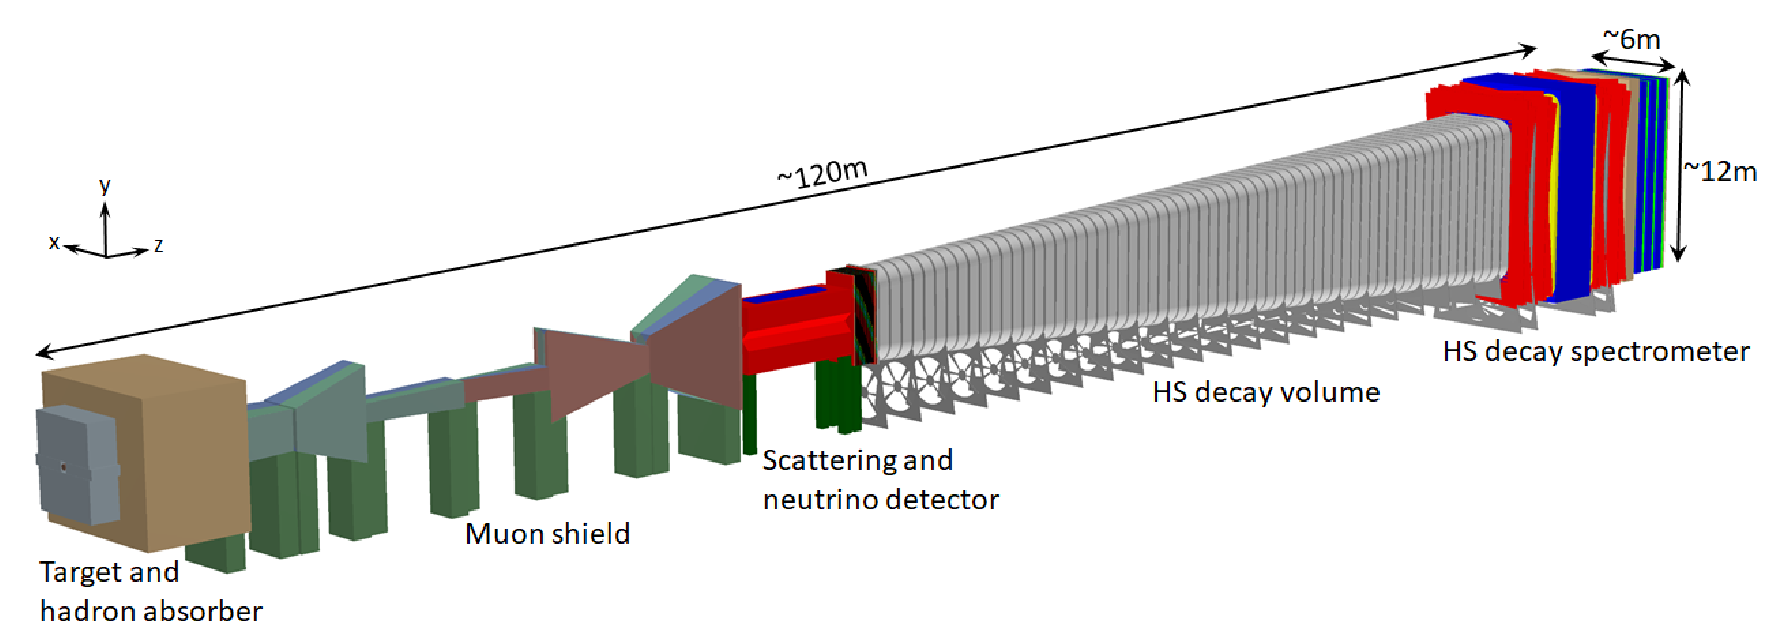
\includegraphics[width=1.\textwidth]{pictures/ship_sketch}
	\caption[Overview of the SHiP experiment.]{Overview of the proposed setup for the SHiP experiment. The target on the left is used as a beam dump for the SPS. Most \ac{sm} particles get absorbed by the hadron absorber directly behind the target. A magnetic muon shield deflects the muon, which will not be absorbed by the hadron absorber, away from the beam line. After the muon shield is a scattering and neutrino detector, and afterward, the \SI{50}{\meter} long decay volume in which non \ac{sm} particles created at the target can decay into \ac{sm} particles. Behind the decay volume, the decay spectrometer is placed. To achieve the zero background goal, the Surround Background Tagger is around the decay volume. \cite{ship_coll}}
	\label{fig:ship_sketch}
\end{figure}

One problem for the measurement is \ac{sm} particles entering the decay volume and getting falsely reconstructed as \ac{hs} events in the spectrometer.
An example of such a background is muons deflected by the muon shield and reflected at the walls of the facility into the decay volume, mimicking the decay products of an \ac{hs} event in the spectrometer.
Therefore it is crucial for the zero background requirement to detect the particles entering the decay volume and tag every event that could be caused by the entering particle as background.
This task is meant to be done by the \ac{sbt}.
As the name suggests, it surrounds the \ac{hs} decay volume, detecting particles entering it.
It is currently in development and this thesis is part of the R\&D effort toward it.
In the following, the \ac{sbt} and the principles of the different parts are described.
The details of the different parts important for this thesis are presented in more detail in the next chapter.

To make the tagging of background events possible and efficient and avoid the incorrect tagging of many \ac{hs} events different pieces of information need to be known about the particles entering the decay volume.
These pieces of information are the energy of the entering particles, the time at which they are entering the decay volume, and the space coordinates at which they are entering.
Therefore the \ac{sbt} is designed as a five-dimensional tagger.
It will consist of approximately 2000 cells that form the walls on the side as well as the top and bottom of the vacuum decay chamber.
The structure is shown in \autoref{fig:sbt}.
In order to fit the overall truncated pyramid shape of the decay volume, the cells have an unsymmetric shape, an example is shown in \autoref{fig:sbt}.
Both of the long edges are parallel, but the shorter sides are not.
The depth of the cells is \SI{20}{\centi\meter} and the wall thickness is planned to be \SI{2}{\centi\meter} \cite{}.
For the detection of particles, a liquid scintillator will be filled into the cells.
A particle passing through one or more cells will deposit energy in the scintillator, causing the emittance of scintillation light.
The amount of emitted light is correlated to the amount of energy deposited in the scintillator.
Two \acp{wom}, PMMA tubes coated with wavelengthshifting paint, are placed in each cell to collect the scintillation light and guide it to an array of \acp{sipm}.
The signals from the \acp{sipm} can be amplified, digitized, and further processed.
Both a \acp{wom} and a \ac{sipm} array are shown in \autoref{fig:sbt}.

\begin{figure}
	\centering
	\begin{subfigure}[b]{0.25\textwidth}
		\centering
		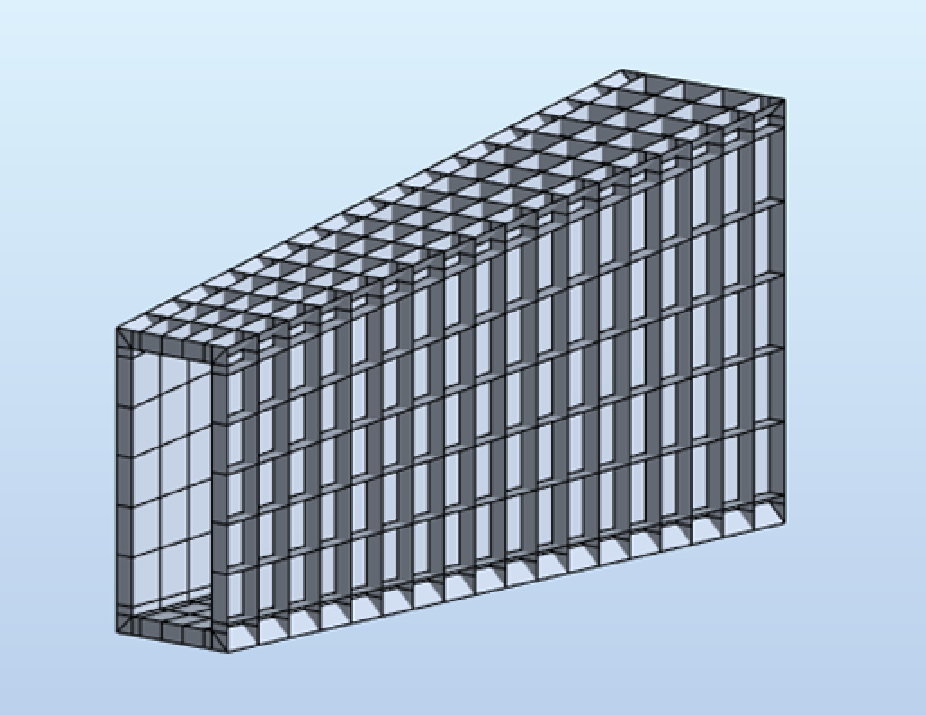
\includegraphics[width=.9\textwidth]{pictures/sbt_structure_sceleton}
		\caption{test}
		\label{fig:sbt_structure_sceleton}
	\end{subfigure}
	\begin{subfigure}[b]{0.25\textwidth}
		\centering
		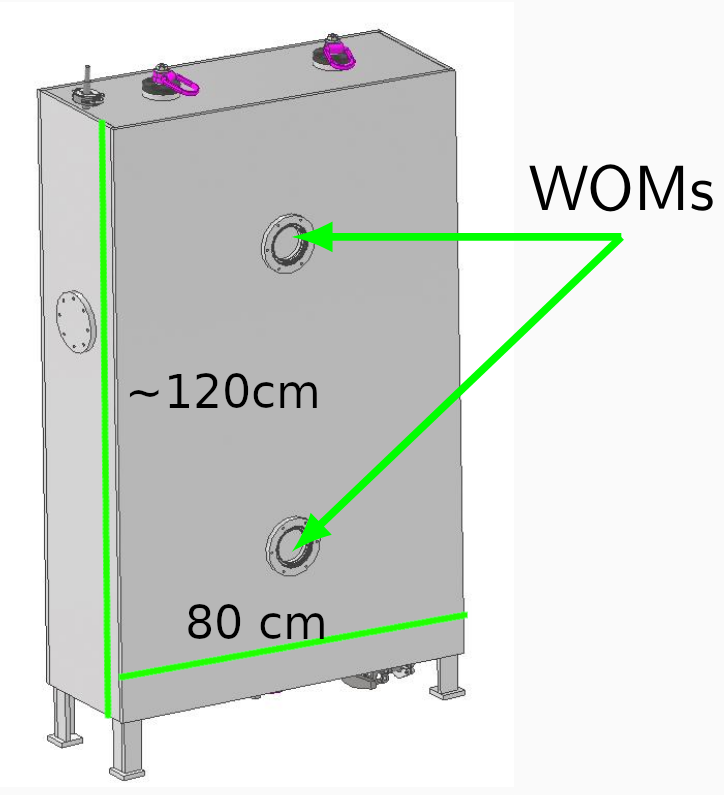
\includegraphics[width=.9\textwidth]{pictures/sbt_structure_cell}
		\caption{test}
		\label{fig:sbt_structure_cell}
	\end{subfigure}
	\begin{subfigure}[b]{0.25\textwidth}
		\centering
		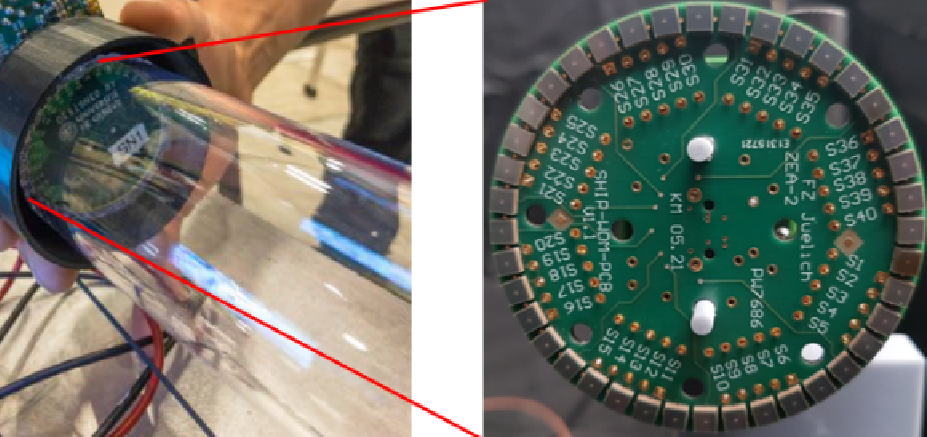
\includegraphics[width=.9\textwidth]{pictures/sbt_structure_wom}
		\label{fig:sbt_structure}
	\end{subfigure}
	\begin{subfigure}[b]{0.25\textwidth}
		\centering
		\includegraphics[width=.9\textwidth]{pictures/sbt_structure_sipm}
		\label{fig:sbt_structure}
	\end{subfigure}
	\caption[Overview of the Surrounding Background Tagger]{The structure of the Surrounding Background Tagger (SBT). Left is the SBT with its approximately 2000 cells. Then the shape of one example cell is shown in b). The light produced by the liquid scintillator inside the cells is captured by two Wavelengthshifting Optical Modules (WOMs) per cell, an example is shown in c), and then guided to an array of Silicon Photomultipliern, shown in d), which will detect the light.}
	\label{fig:sbt}
\end{figure}

This thesis is in the scope of the R\&D of the \ac{sbt}.
For the R\&D of the \ac{sbt}, a prototype of one of the cells was built, with which important parts can be tested.
Starting from the cell's material itself, a reflecting coating on the inside of the cell, the coated \acp{wom}, and the \acp{sipm} to name a few.
This thesis is about the readout of the \acp{wom} of the prototype.
Since the \ac{asic} meant to be used for the readout in the \ac{sbt} is in development by the Forschungszentrum Jülich and not yet finished, another readout is needed for the One Cell Prototype in order to test it.
The next chapter presents the One Cell Prototype with the focus on the \ac{wom} readout.



\appendix

\chapter{List of acronyms}
\begin{acronym}[SiPM]
    \acro{sm}[SM]{Standard Model}
    \acro{lhc}[LHC]{Large Hadron Colider}
    \acro{ship}[SHiP]{Search for Hidden Particle}
    \acro{sps}[SPS]{Super Proton Synchrotron}
    \acro{sbt}[SBT]{Surround Background Tagger}
    \acro{sipm}[SiPM]{Silicon Photomultiplier}
    \acro{pcb}[PCB]{Printed Circuit Board}
    \acro{asic}[ASIC]{Application Specific Integrated Circuit}
    \acro{dac}[DAC]{Digital to Analog Converter}
    \acro{adc}[ADC]{Analog to Digital Converter}
    \acro{apd}[APD]{Avalanche Photodiode}
    \acro{daq}[DAQ]{Data Acquisition}
    \acro{wom}[WOM]{Wavelengthshifting Optical Module}
    \acro{spad}[SPAD]{Single Photon Avalanche Diode}
    \acro{dc}[DC]{Dark Count}
    \acro{dcr}[DCR]{Dark Count Rate}
    \acro{fpga}[FPGA]{Field Programmable Gate Array}
\end{acronym}

\chapter{Slow Control Settings}
\begin{table}[h]
    \centering
    \caption[Slow control settings]{Slow control settings used for the measurements. In the first column the slow control parameters are listed. The corresponding slow control bits are listed in the second column, and the values set for the bits are listed in the third column. In the last column are the corresponding physical values as far as they are known.}
    \label{tab:sc_settings}
    \begin{tabularx}{1.\textwidth}{>{\raggedright\arraybackslash}X|>{\centering\arraybackslash}X|>{\centering\arraybackslash}X|>{\centering\arraybackslash}X}
        parameter & slow control bit & bit value & physical value \\\hline\hline
        preampifier ch0 &  & \multirow{8}{*}{111110 [62]} & \multirow{8}{*}{\SI[per-mode=symbol]{60}{\volt\per\volt}} \\
        preampifier ch4 &  &  &  \\
        preampifier ch8 &  &  &  \\
        preampifier ch12 &  &  &  \\
        preampifier ch16 &  &  &  \\
        preampifier ch20 &  &  &  \\
        preampifier ch24 &  &  &  \\
        preampifier ch28 &  &  &  \\\hline
        slow shaper ch0 &  & \multirow{8}{*}{6} & \multirow{8}{*}{\SI{12.5}{\nano\second}} \\
        slow shaper ch4 &  &  &  \\
        slow shaper ch8 &  &  &  \\
        slow shaper ch12 &  &  &  \\
        slow shaper ch16 &  &  &  \\
        slow shaper ch20 &  &  &  \\
        slow shaper ch24 &  &  &  \\
        slow shaper ch28 &  &  &  \\\hline
         &  &  & 
        \end{tabularx}
\end{table}

\newpage
\listoffigures

\newpage

\listoftables
\newpage

\begin{thebibliography}{9}
\bibitem{ship} SHiP - Search for Hidden Particles, \url{https://ship.web.cern.ch/}, June 2022
\bibitem{ship_facility} S. Alekhin et al ``A facility to search for hidden particles at the CERN SPS: the SHiP physics case'', Rep. Prog. Phys. 79, Oct 2016, \url{https://doi.org/10.1088/0034-4885/79/12/124201}
\bibitem{ship_coll} SHiP Collaboration, ``SPS Beam Dump Facility - Comprehensive Design Study'', 2020, arXiv:1912.06356
\bibitem{kemp} J. Kemp, ``Development of a silicon photomultiplier based scintillator detector for cosmic air showers'' Phd thesis, Dez 2020, RWTH Aachen
\bibitem{nucl} F. Acerbi, S. Gundacker, ``Understanding and simulating SiPMs'', NIM-A vol. 926, p. 16-35, 2019. doi: 10.1016/j.nima.2018.11.118
\bibitem{HAMA_mppc} Hamamatsu Photonics, MPPC, \url{https://www.hamamatsu.com/content/dam/hamamatsu-photonics/sites/documents/99_SALES_LIBRARY/ssd/mppc_kapd9005e.pdf}, date: 20.06.2022
\bibitem{HAMsipm_ds} Hamamatsu S14160-3050HS Datasheet,
\url{https://www.hamamatsu.com/content/dam/hamamatsu-photonics/sites/documents/99_SALES_LIBRARY/ssd/s14160_s14161_series_kapd1064e.pdf}, date: 05.05.2022

\bibitem{citiroc} Weeroc Citiroc 1A Datasheet V2.5, \url{https://www.weeroc.com/my-weeroc/download-center/citiroc-1a/16-citiroc1a-datasheet-v2-5/file}, date: 09.05.2022 
\bibitem{bsc_jonathan} J. Grieshaber, ``Calculation and simulation of Silicon photomultiplier signals'', B.Sc. thesis, Feb 2022, ALU Freiburg
\end{thebibliography}




\end{document}
